\chapter{Założenia projektowe}
\section{Wymagania funkcjonalne}
Sposób zachowania oraz oczekiwane funkcje gry opisano w poniższych podrozdziałach.
\subsection{Reguły i mechanika gry}
Gra stworzona w ramach projektu będzie nazywała się \emph{Sunset Showdown}. Charakterystyczne dla gry będzie ujednolicenie postaci sterowanymi przez graczy. Każda z postaci będzie miała 3~punkty zdrowia, a zwycięstwo w rundzie będzie osiągane poprzez zredukowanie zdrowia przeciwnika do zera. W przypadku trzykrotnego powodzenia tego procesu, gracz wygrywa całą grę. 

Postacie będą miały możliwość zadawania ciosów na trzech różnych wysokościach: \emph{high} (cios wysoki), \emph{mid} (cios wyprowadzony w środkową część ciała) oraz \emph{low} (cios niski). Wysokość ciosu wpływa na to, w jakim stanie można go zablokować lub uniknąć. Cios \emph{high} można zablokować stojąc, uniknąć zaś kucając. Cios \emph{mid} można zablokować w pozycji stojącej, jednak nie chroni przed nim kucanie. Natomiast ciosem \emph{low} można trafić stojącego przeciwnika, przy czym może on go zablokować kucając. Dodatkowo, każdy cios będzie zadawany z inną szybkością. Atak \emph{high} będzie najszybszy, \emph{mid} zajmie środkową pozycję, natomiast cios \emph{low} będzie najwolniejszy. 

Każdy atak zadaje określoną ilość obrażeń (\emph{high} -- 3 obr., \emph{mid} -- 2 obr., \emph{low} -- 1 obr.). Dodatkowo każdy cios będzie powodował inną animację u przeciwnika na bloku (tzw.~\emph{blockstun}), od której będzie zależało, jak będzie wyglądała sytuacja po zablokowanym ataku. Po zablokowaniu ataku \emph{high}, atakujący znajduje się w lepszej pozycji, gdyż \emph{blockstun} trwa na tyle długo, że atakujący będzie mógł szybciej odzyskać kontrolę nad postacią. W przypadku ataku \emph{mid}, sytuacja odwraca się, a po zablokowaniu obrońca znajduje się w lepszej pozycji. Sytuacja po zablokowaniu ciosu \emph{low} jest szczególnie dynamiczna, ponieważ blokujący ma wystarczająco dużo czasu, aby zareagować ciosem \emph{high}, co równa się z wygraniem rundy (tzw.~\emph{block punishment}).

Wszystkie kluczowe informacje na temat ciosów postaci znajdują się w tabeli~\ref{tab:ataki}. Wartości szybkości ruchów i sytuacji zarówno na trafieniu i na bloku są podawane w ,,klatkach'', które są równoznaczne z 1/60 sekundy (np.\ jeżeli sytuacja na trafieniu wynosi +2 oznacza to że postać atakującego po trafieniu będzie mogła wrócić do kontroli nad swoją postacią o 2/60 sekundy szybciej niż przeciwnik).

\begin{table}[htb] \small
\centering
\caption{Atrybuty ataków dostępnych dla postaci}
\label{tab:ataki}
\begin{tabularx}{\linewidth}{|c|c|c|c|>{\centering\arraybackslash}X|} \hline\
Wysokość ataku & Szybkość ataku & Obrażenia & Sytuacja na bloku & Sytuacja na trafieniu \\ \hline\hline
\texttt{high} & 15 & 3 & +1 & nie dotyczy \\ \hline
\texttt{mid} & 18 & 2 & -2 & +2\\ \hline
\texttt{low} & 21 & 1 & -15 & +2\\ \hline
\end{tabularx}
\end{table}

\subsection{Interfejs użytkownika}
Na rysunku \ref{fig:interfejs} przedstawiono wygląd interfejsu użytkownika gry \emph{Sunset Showdown}. Postacie graczy zobrazowane są na nim jako sylwetki w jednolitym, czarnym kolorze. W górnej części ekranu znajdują się zielone paski zdrowia dla każdego z graczy. Zmniejszają się one w miarę otrzymywania obrażeń przez postacie. Poniżej pasków zdrowia znajdują się ikony w kształcie kółek. Jeżeli są zapalone na żółto, to wskazują na wygrane rundy.
\begin{figure}[htb]
	\centering
		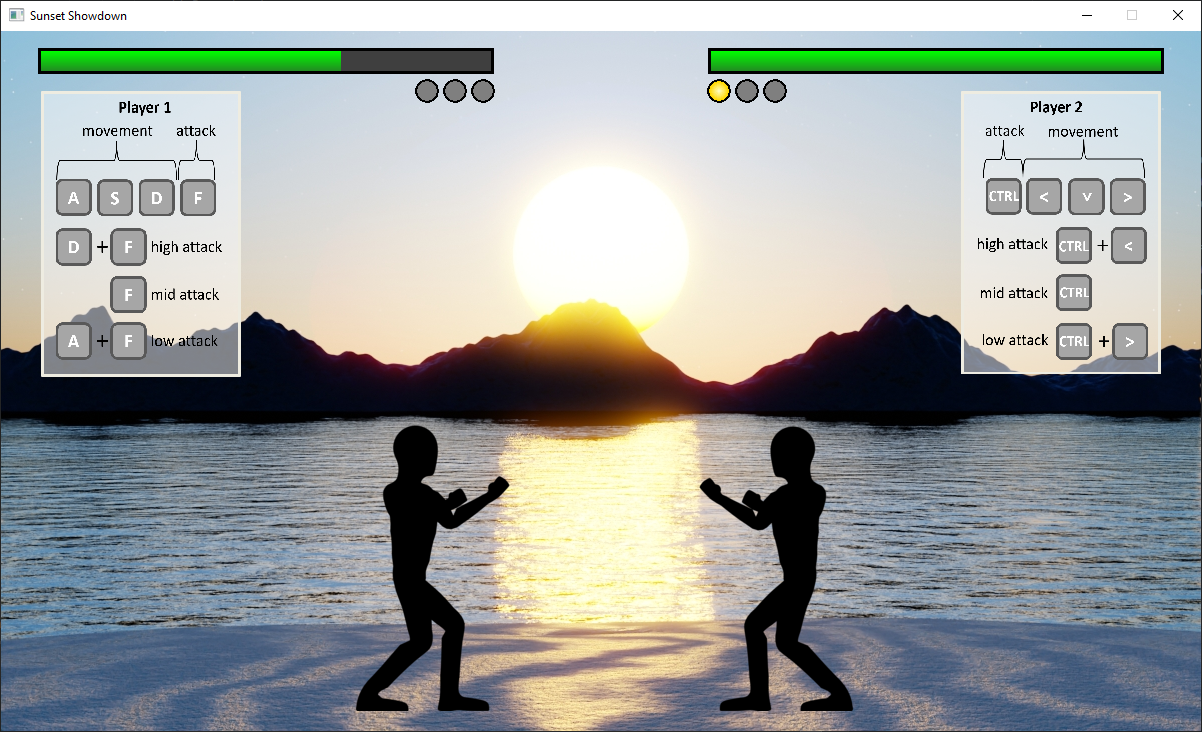
\includegraphics[width=0.64\linewidth]{rys02/interfejs}
	\caption{Widok intefejsu użytkownika gry \emph{Sunset Showdown}}
	\label{fig:interfejs}
\end{figure}

Po bokach ekranu umiejscowione są schematy sterowania dla każdego z graczy, przedstawiające przypisane klawisze i ich funkcje w grze. Dla Gracza 1, po lewej stronie, przyciski 'A', 'S', 'D', i 'F' odpowiadają za ruchy i podstawowe ataki, z dodatkowymi kombinacjami klawiszy dla ataków wysokich, średnich i niskich. Analogicznie, Gracz 2, po prawej stronie ekranu, korzysta z klawiszy strzałek oraz 'CTRL' do sterowania swoją postacią i wykonania ataków.

\subsection{Tryby gry}
W \emph{Sunset Showdown} dostępne będą dwa podstawowe tryby gry. Tryb offline umożliwi dwóm graczom wspólną rozgrywkę na jednym komputerze przy użyciu tej samej klawiatury. Oprócz tego gra będzie oferować tryb online, który pozwoli graczom na połączenie się przez Internet z~osobnych komputerów. W tym trybie gracze będą mogli tworzyć pokoje gry, do których dostęp jest możliwy po wprowadzeniu specjalnego kodu pokoju. Funkcje te będą dostępne w menu głównym gry.

\section{Wymagania niefunkcjonalne}
W niniejszym podrozdziale zebrano wymagania niefunkcjonalne, w tym wymagania odnośnie wykorzystanych narzędzi i technologii oraz wymagania systemowe.

\subsection{Narzędzia i technologie}
Projekt gry zostanie zrealizowany w języku Java \cite{Java}, z wykorzystaniem Java Development Kit (JDK) wersja 17.
Dodatkowo wykorzystany zostanie framework LibGDX \cite{LibGDX}. Framework ten będzie odpowiedzialny za szereg funkcji, takich jak ładowanie zasobów, wyświetlanie sprite'ów, odtwarzanie dźwięków, a także zarządzanie główną pętlą gry i interfejsem użytkownika w systemie Windows. 

Do serializacji danych zastosowana zostanie biblioteka Kryo \cite{Kryo}, natomiast aspekty sieciowe obsłuży Kryonet \cite{Kryonet} wraz z biblioteką weupnp \cite{weupnp}. Ponadto, do stworzenia pomocniczego programu przeznaczonego do generowania plików JSON, które szczegółowo opisują ruchy postaci, wykorzystam bibliotekę JavaFX \cite{JavaFX}. 

Proces tworzenia modeli 3D i ich animacji, zarówno dla postaci, jak i tła, zostanie wykonany przy użyciu programu Blender \cite{Blender}. Natomiast do kreowania spritesheet'ów wybór padł na ImageMagick \cite{ImageMagick}. Ostatnią częścią projektu będzie udźwiękowienie gry, do czego posłużą darmowe dźwięki pobrane ze strony pixabay \cite{Pixabay}. 


\subsection{Wymagania systemowe}
Aby uruchomić grę, konieczne jest posiadanie komputera z systemem operacyjnym Windows (najlepiej Windows 10). Do wykorzystania trybu online niezbędne jest połączenie z internetem. W przypadku pełnienia roli hosta (założyciela pokoju dołączanego przez innych graczy), wymagana jest odpowiednia konfiguracja sieciowa: komputer musi być połączony z routerem, który z kolei powinien być bezpośrednio podłączony do dostawcy usług internetowych (ISP). Istotna jest również aktywna funkcja Universal Plug and Play (UPnP) na routerze, umożliwiająca automatyczne przekierowywanie portów. Minimalne wymagania sprzętowe:
\begin{itemize}
\item procesor -- AMD Ryzen 3 2200U,
\item karta graficzna -- AMD Radeon Vega3 Mobile Graphics,
\item pamięć RAM: -- 8 GB,
\item wolne miejsce na dysku -- 200 MB.
\end{itemize}

\subsection{Środowisko programistyczne}
W przypadku decyzji o uruchomieniu aplikacji poprzez skompilowanie dostępnego w publicznym repozytorium kodu źródłowego, konieczne będzie spełnienie dodatkowych wymagań infrastrukturalnych. Do nich należą:
\begin{itemize}
\item zintegrowane środowisko programistyczne (IDE) -- zalecane Intellij IDEA \cite{IntellijIDEA}; 
\item system zarządzania projektami i zależnościami -- Gradle,
\item system wersjonowania kodu -- platformy GitHub \cite{GitHub} oraz program git \cite{Git}.
\end{itemize}
Po otwarciu projektu w IDE, pozostałe zależności powinny zostać automatycznie pobrane. Ważne jest również, aby upewnić się, że folder roboczy uruchamianej aplikacji jest folderem assets znajdującym się bezpośrednio w głównym katalogu projektu.

